% This must be in the first 5 lines to tell arXiv to use pdfLaTeX, which is strongly recommended.
\pdfoutput=1
% In particular, the hyperref package requires pdfLaTeX in order to break URLs across lines.

\documentclass[11pt]{article}

% Remove the "review" option to generate the final version.
\usepackage[final]{ACL2023}

% Standard package includes
\usepackage{times}
\usepackage{latexsym}
\usepackage{float}
\usepackage{graphicx}
\usepackage{tabularx}

% For proper rendering and hyphenation of words containing Latin characters (including in bib files)
\usepackage[T1]{fontenc}
% For Vietnamese characters
% \usepackage[T5]{fontenc}
% See https://www.latex-project.org/help/documentation/encguide.pdf for other character sets

% This assumes your files are encoded as UTF8
\usepackage[utf8]{inputenc}

% This is not strictly necessary, and may be commented out.
% However, it will improve the layout of the manuscript,
% and will typically save some space.
\usepackage{microtype}

% This is also not strictly necessary, and may be commented out.
% However, it will improve the aesthetics of text in
% the typewriter font.
\usepackage{inconsolata}


% If the title and author information does not fit in the area allocated, uncomment the following
%
%\setlength\titlebox{<dim>}
%
% and set <dim> to something 5cm or larger.

\title{Empowering the Fact Checkers: Automatic Identification of Claim Spans on Twitter}

% Author information can be set in various styles:
% For several authors from the same institution:
% \author{Author 1 \and ... \and Author n \\
%         Address line \\ ... \\ Address line}
% if the names do not fit well on one line use
%         Author 1 \\ {\bf Author 2} \\ ... \\ {\bf Author n} \\
% For authors from different institutions:
% \author{Author 1 \\ Address line \\  ... \\ Address line
%         \And  ... \And
%         Author n \\ Address line \\ ... \\ Address line}
% To start a seperate ``row'' of authors use \AND, as in
% \author{Author 1 \\ Address line \\  ... \\ Address line
%         \AND
%         Author 2 \\ Address line \\ ... \\ Address line \And
%         Author 3 \\ Address line \\ ... \\ Address line}


\author{Joseph Picchi, Shiyao Guo, Yuning Yang \\
        University of California, Los Angeles \\
        \texttt{jpicchi22@g.ucla.edu}, \texttt{sguo18@g.ucla.edu}, \texttt{yuningyang@g.ucla.edu}
        }
        
% \author{ Joseph Picchi, \\
%   Affiliation / Address line 1 \\
%   Affiliation / Address line 2 \\
%   Affiliation / Address line 3 \\
%   \texttt{jpicchi22@g.ucla.edu} \\\And
%   Second Author \\
%   Affiliation / Address line 1 \\
%   Affiliation / Address line 2 \\
%   Affiliation / Address line 3 \\
%   \texttt{email@domain} \\}

\begin{document}
\maketitle
\begin{abstract}
During the COVID pandemic, the prevalence of fake news and misinformation caused fear, anxiety, and social unrest, underscoring the need for wide-scale fact checking. We seek to assist human fact checkers by automatically extracting spans of text that represent claims in COVID-related tweets. To do so, we developed large language models to perform automatic claim span detection. We attemped the task with several models. Our encoder models (Bert, DeBERTa, DistilBert, and BERT+LSTM) yielded state-of-the art results for the dataset provided, while our encoder-decoder models (T5 and BART) achieved more modest performance. The superior performance of DeBERTa relative to all of the other models we tested is consistent with previous literature addressing this task and datset.
\end{abstract}

\section{Introduction}

The rise of social media and internet-based communications mediums has accelerated the spread of (mis)information. Prior research finds that the often-novel nature of fake news encourages users to share it more frequently than real news, causing misinformation to spread more rapidly than true information online \cite{false-news-spreads}.

Fact checkers aim to combat misinformation. Most claim verification is performed manually, making it imperative to assist human fact-checkers as much as possible \cite{fact-checking-is-manual}. Our research seeks to assist them by training natural language models to automatically identify claims made in social media posts.

In particular, we fine-tune encoder and encoder-decoder models on a Twitter corpus of 7.5K tokenized tweets annotated with the corresponding claims they make. An example is shown in figure-\ref{fig: 1-tweet}. Each example can have one or more claims.

\begin{figure}[]
    \centering
    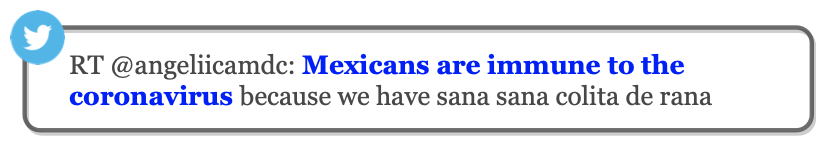
\includegraphics[width=7cm]{images/1-tweet.png}
    \caption{A COVID-related tweet with the claim span highlighted in blue. See appendix figure- for more examples}
    \label{fig: 1-tweet}
\end{figure}

The task was originally defined by \cite{empowering-the-fact-checkers}, which created the dataset, formalized the task, and defined a claim as “an assertion that deserves our attention” \cite{claim-definition-1} and “is the key component of any argument” \cite{claim-definition-2}. The dataset was then posted publicly in a Codalab challenge\footnote{\href{https://codalab.lisn.upsaclay.fr/competitions/13099}{"Empowering the Fact-checkers! Automatic Identification of Claim Spans on Twitter"}}.

\subsection{Previous Work}

Previous work has focused on 3 main claim-oriented research areas: detection \cite{detection-research-area}, check worthiness \cite{check-worthiness}, and verification \cite{verification}. Within the claim detection area, researchers have developed course-grained sentence-level claim detection models (Chakrabarty et al. (2019); \cite{detection-research-area, claim-detection}. Few works have focused on fine-grained span detection within s entences for COVID-related tweets.

Previous conferences \cite{conference-pipeline} have underscored the importance of claim span detection in fact checking by identifying 4 fundamental steps in the pipeline of end-to-end AI fact checking: (1) identifying claims, (2) detecting previously fact-checked claims, (3) retrieving evidence, and (4) verifying the claim. Within these areas, most research has focused on downstream tasks (2)-(4), such as \cite{downstream-tasks} that takes an input sentence and generates a ranked list of previously fact-checked claims to verify it.

In the area of span identification, researchers have developed fine-grained models to extract spans in other domains like toxic language \cite{toxic-language}, propaganda \cite{propaganda}, and hate speech \cite{hate-speech}. Such studies have tested various methods, including transformers, data augmentation, and ensembling.

For our specific task of fine-grained span identification for COVID tweets, encoder-only models were developed by the paper that developed the dataset and defined the task \cite{empowering-the-fact-checkers}, including DistilBERT, BERT, SpanBERT, RoBERTA, DABERTa, and a BiLSTM. Our research builds upon this progress by fine-tuning more recent checkpoints of BERT and its variants, and by attempting the task with a BERT+LSTM model and several encoder-decoder models.

\section{Methods}
\subsection{Encoder-Decoder Models}
Although the claim span identification task is more naturally formulated as a token identification task, \cite{T5-paper} have demonstrated that many NLP tasks can be reformulated in a sequence to sequence format. So we designed multiple seq2seq input-output formats for our task and used them to fine tune T5 and BART. The motivation was to test whether transfer learning from T5 could improve predictions for claim span detection.

We fine-tuned T5 with 2 different input formats. The first format structures claim span detection as a Q\&A task to take advantage of T5’s text extraction capabilities in its pre-trained Q\&A task. The second format structures claim span detection as a new task type that wasn’t seen in pre-trianing. Inputs are structured as “Extract the claims: [tweet text]”. Both input formats have the same output format: claims are listed as consecutive sentences.

BART was fine-tuned only on the second input format, since it’s not pre-trained on T5’s Q\&A task.

To evaluate the sequence-to-sequence models, we used Rouge 1, 2, L, and Lsum metrics that score predictions based on the number of shared words with the example label \cite{rouge}. Analysis of the rougeL and Lsum scores also ensures that the overlapping words occur in the same consecutive sequence in both the prediction and the label, thus ensuring that a coherent subset or superset of the target claim is properly extracted.

\subsection{Encoder Models}
This is essentially a name entity recognization task, which is also known as NER. NER requires BIO tagging for each token, but the training and test data do not have BIO tagging. So we preprocessed the training and test data by adding BIO tagging to each token. For token that is  the start of the claim, we labelled it using B. For token that is inside the claim, we labelled it using I. For all the rest of the tokens, we label them as O.

After data preprocessing, we created a function called convert\_to\_input, which returns the input to different BERT models. We used a tokenizer to tokenize each token and then converted them into ids. We also set the attention mask to focus on tokens with B and I tagging.

We tried several BERT models, namely BERT, DistilBert, and DABerta. For optimizer, we used AdamW. There are 3 inputs into the models, namely tokens in the form of ids, the labels, and the attention masks.

In addition to the BERT models, we also experimented with a hybrid LSTM+BERT model. In this model, we first used BERT to generate context-aware embeddings for each token in the input. These embeddings were then passed to a bidirectional LSTM, which processed the sequence of embeddings over time. The LSTM, being a type of recurrent neural network, is effective at capturing long-term dependencies in sequence data, which is beneficial in NER tasks where the classification of a word can depend on the words that precede it in a sentence.

However, LSTMs can suffer from a short-sighted vantage wherein they place greater consideration upon prior outputs that were generated more recently when predicting new outputs. To mitigate this, we used the bidirectional variant of LSTM, which processes the data in both directions (forward and backward) and can capture information from both past and future states. The goal of this hybrid LSTM+BERT model was to leverage the strengths of both models and provide a robust approach to the NER task.

\section{Results}

\subsection{Encoder-Decoder Models}

% subset of entire dev set
% entire dev set
\begin{table}[]
% \centering
\begin{tabular}{l c c c}
\hline
\textbf{Metric} & \textbf{T5 QA} & \textbf{T5} & \textbf{BART}\\
\hline
Rouge1 Fmeasure & 0.780 & 0.775 & 0.775\\
RougeL Fmeasure & 0.776 & 0.772 & 0.771\\
\hline
\end{tabular}

\caption{Sequence-to-sequence model performance: All 3 encoder-decoder models achieved approximately equivalent performance, irregardless of architecture or input formulation. Note that "T5" is the T5 model fine-tuned without the Q\&A input formulation. See appendix table-\ref{tab appendix seq2seq: general} for the full results.}
\label{tab seq2seq: general}
\end{table}

Table-\ref{tab seq2seq: general} indicates that T5 performed nearly equivalently on both input formats, with slightly better performance on the Q\&A format across all metrics. This indicates that Q\&A pre-training of T5 yielded minimal benefits for this task.

BART performed negligibly worse than T5 on the same non-Q\&A input format. Their near-equivalent performance indicates that transfer learning with T5 produced almost no performance boost for this task.

All 3 encoder-decoder models performed considerably worse than BERT, indicating that any benefits of transfer learning were outweighed by the suboptimal sequence-to-sequence formulation of the task. The lower performance can be explained by the difference in objective between encoder and encoder-decoder models.

Encoder-decoder models optimize the probability of each output token given the input sequence and preceding output tokens. This objective is suboptimal because our task seeks to classify each token as a claim or non-claim solely based on the input sequence and irrespective of other tokens previously outputted by the decoder. This is particularly erroneous because some tweets have multiple claim spans. Since each claim is independent, tokens outputted for the second claim should not probabilistically depend on tokens outputted for the first claim. Table-\ref{tab seq2seq: claims} evidences this explanation by showing that the T5 model achieved much higher F1 scores on tweets with one claim compared to tweets with multiple claims.

% one tweet vs multiple tweets --> abbridged



\begin{table}[]
% \centering
\begin{tabular}{l c c}
\hline
\textbf{Metric} & \textbf{1 Claim} & \textbf{2+ Claims}\\
\hline
Rouge1 Fmeasure & 0.829 & 0.600\\
\phantom{X}Rouge1 Precision & 0.875 & 0.876\\
\phantom{X}Rouge1 Recall & 0.817 & 0.481\\
RougeL Fmeasure & 0.826 & 0.592\\
\phantom{X}RougeL Precision & 0.872 & 0.864\\
\phantom{X}RougeL Recall & 0.814 & 0.475\\
\hline
\end{tabular}

\caption{One claim vs. multiple claims: The T5 Q\&A model achieves significantly higher Fmeasure and recall scores on examples where the tweet makes one claim compared to examples where the tweet makes more than one claim. See appendix table-\ref{tab appendix seq2seq: claims} for the full results.}
\label{tab seq2seq: claims}
\end{table}

In contrast, the encoder objective optimizes the contextual representation of each token. This is more desirable for our task because it optimizes the independent classification of each token as a claim or non-claim based on the input sequence. This explains the superior performance of our BERT models.

Interestingly, table-\ref{tab seq2seq: general} shows that the Rouge1 Fmeasure is approximately equivalent to the RoughL Fmeasure for all models. This indicates that nearly all words shared between the model predictions and reference labels appear consecutively in the prediction text. Thus, the model is at least able to extract a subset or superset of the actual claim text, as opposed to randomly-sequenced words that happen to appear in the reference text.

\begin{table}
    % \centering
    \begin{tabular}{p{2.8in}}
    \hline
    \textbf{Label: }\\
    \hline
    US \&amp; China Collaborated to Make a Deadly \#Corona\textcolor{red}{virus. Dr Fauci knew it was being developed as a \#bioweapon.} \\
    \hline
    \textbf{Prediction: } \\
    \hline
    US \&amp; China Collaborated to Make a Deadly \#Corona \\
    \hline
    
    \end{tabular}
    
    \caption{Labels vs predictions for multi-claim tweets: T5 consistently predicts a subset of the claim text from the labels for examples in which the tweet makes more than one claim. See appendix table-\ref{tab appendix seq2seq: label prediction pairs} for more examples.}
    \label{tab seq2seq: label prediction pairs}
\end{table}

Lastly, table-\ref{tab seq2seq: claims} indicates that the Rouge precision was much greater than recall for examples with multiple claims, whereas precision and recall were approximately equivalent for examples with one claim. This indicates that the ratio of prediction-label shared words to prediction words is much greater than the ratio of prediction-label shared words to label words. Thus, for examples with multiple claims, T5 routinely predicts a subset of the claim text in the labels. We verify this by manually examining poorly predicted examples that make multiple claims. One such example is shown in table-\ref{tab seq2seq: label prediction pairs}. Moreover, the subset that T5 predicts typically begins at the start of the label. This further evidences the fact that the learning objective of encoder-decoder models is suboptimal for our task because each claim in the same tweet is independent of the others. Thus, tokens outputted for the second claim should not depend on tokens outputted earlier for the first claim.

% % examples of predictions and labels for examples that make multiple claims --> abridged
% \begin{table}[]
% % \centering
% \begin{tabular}{l c c c}
% \hline
% \textbf{Metric} & \textbf{BERT} & \textbf{DistilBert} & \textbf{Deberta}\\
% \hline
% Precision & 0.9979 & 0.9973 & 0.9986\\
% Recall & 0.9979 & 0.9973 & 0.9986\\
% F1 Score & 0.9979 & 0.9973 & 0.9986\\
% \hline
% \end{tabular}

% \caption{ Bert models performance see appendix for the full results.}
% \label{tab seq2seq: general}
% \end{table}

% examples of predictions and labels for examples that make multiple claims --> abridged
\begin{table}[]
% \centering
\begin{tabular}{l c c c}
\hline
\textbf{Model} & \textbf{Precision} & \textbf{Recall} & \textbf{F1}\\
\hline
BERT & 0.998 & 0.998 & 0.998 \\
DistilBERT & 0.997 & 0.997 & 0.997 \\
DeBERTa & 0.999 & 0.999 & 0.999 \\
BERT+LSTM & 0.760 & 0.760 & 0.760 \\
\hline
\end{tabular}

\caption{Encoder model performance: The LSTM detracted from BERT's predictions, and all other BERT models achieved state-of-the-art performance for the given dataset.}
\label{tab encoder: general}
\end{table}

\subsection{Encoder Models}
We used f1 score, precision, and recall as metrics to measure the performance of our model. Since the test dataset is not provided and the only two datasets available are train dataset and dev dataset, we used dev dataset as our test dataset. All of our BERT models have really high F1 score, precision, and recall. But the best performing model is DABerta, which correspond to the paper’s finding that DABerta yielded the best results in this automatic identification of claim spans on twitter task. We tuned the hyper parameters and found out that setting the learning rate to 1e-5 and setting the batch size to 32 had the best performance.

We also experimented with a hybrid LSTM+BERT model. However, this model achieved a lower F1 score of 0.7601. This suggests that the addition of the LSTM layer did not improve performance for this particular task. In fact, it may have introduced additional complexity that hindered the model's ability to accurately identify claim spans.

While BERT is able to consider the context from both directions for each token, LSTM processes the sequence in a linear fashion. This difference in handling sequence data might have contributed to the lower performance of the LSTM+BERT model. Additionally, the LSTM layer adds more parameters to the model, which could make the model more prone to overfitting, especially if the amount of training data is limited.

Despite the lower performance of the LSTM+BERT model compared to the BERT and DeBerta models, it's worth noting that an F1 score of 0.7601 is still reasonably good. The LSTM+BERT model could potentially be improved with further tuning and optimization. Future work could explore different ways of combining BERT and LSTM, or investigate other types of recurrent layers or architectures.



\section{Conclusion}

In this study, we explored various models for the task of Claim Span Detection, aiming to accurately identify the beginning and end of a claim within a sentence. Our models included both sequence-to-sequence models (T5 and BART) and encoder models (BERT, DABerta, DistilBert, and a hybrid LSTM+BERT model).

Our results showed that the encoder models generally outperformed the sequence-to-sequence models. This is likely due to the fact that the encoder models optimize the contextual representation of each token, which is more suitable for our task of classifying each token as a claim or non-claim based on the input sequence. On the other hand, sequence-to-sequence models optimize the probability of each output token given the input sequence and preceding output tokens, which is not ideal for our task as it does not consider the independence of each claim in the same tweet.

Among the encoder models, DABerta achieved the highest performance, with an F1 score close to 0.99. This aligns with existing literature that suggests DABerta's superior performance in the task of automatic identification of claim spans on Twitter. The hybrid LSTM+BERT model, while not performing as well as the other encoder models, still achieved a respectable F1 score of 0.7601, suggesting potential for further optimization and tuning.

We release our code\footnote{\href{https://github.com/jpicchi18/NLP-claim-span-detection}{NLP-claim-span-detection}} for the purposes of reproducibility, demonstration, and further experimentation.

\subsection{Future Work}

While our models achieved high performance, there is still room for improvement and exploration. For the sequence-to-sequence models, future work could investigate different input-output formats or explore other types of sequence-to-sequence architectures. For the encoder models, future work could explore different ways of combining BERT and LSTM, or investigate other types of recurrent layers or architectures.

Furthermore, the performance of the models could potentially be improved by fine-tuning the hyperparameters, such as the learning rate and batch size. It would also be interesting to investigate the use of other optimization algorithms besides AdamW.

\section*{Acknowledgements}
Our team would like to acknowledge the teaching staff of the UCLA COM SCI 263 course for helping us learn the skills and knowledge demonstrated in this project. This includes instructor Kai-Wei Chang and teaching assistants Tanmay Parekh, Elaine Wan, and Masoud Monajatipoor.

We also acknowledge \cite{empowering-the-fact-checkers} for laying the groundwork and creating the dataset for this task.

% Entries for the entire Anthology, followed by custom entries
\bibliography{anthology,custom}
\bibliographystyle{acl_natbib}

\appendix

\section*{Appendix}
\section{Task Structure}
This section contains additional information about the structure of claim span identification task and the nature of the inputs that our models processed.

\begin{figure}[H]
    \centering
    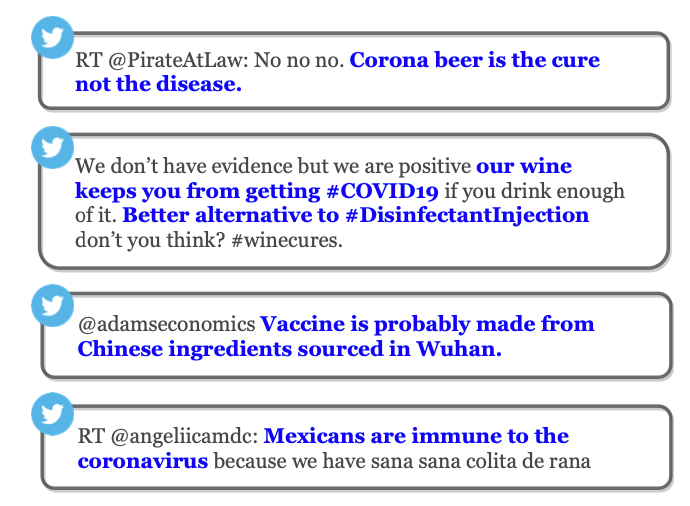
\includegraphics[width=7cm]{images/4-tweets.png}
    \caption{COVID-related tweets from the training dataset with claim spans highlighted in blue.}
    \label{fig appendix: 4-tweets}
\end{figure}

\begin{table}[H]
% \centering
\begin{tabular}{p{2.8in}}
\hline
\textbf{Tokens:} ['If', ' you', ' swam', ' in', ' buckeye', ' lake', ' as', ' a', ' kid', ' you', ' are', ' immune', ' to', ' the', ' coronavirus'] \\
\textbf{Start Indices:} [0]\\
\textbf{End Indices:} [14]\\

\hline\hline

\textbf{Tokens:} ['RT', ' \@FirebaughNorman', ': Tom', ' Cotton', ' was', ' right', ': The', ' Wuhan', ' virus', ' probably', ' came', ' from', ' a', ' bioweapons', ' lab']\\
\textbf{Start Indices:} [2, 6]\\
\textbf{End Indices:} [5, 14]\\

\hline\hline

\textbf{Tokens:} ['In', ' all', ' fairness', ', injecting', ' \#lysol', ' or', ' \#bleach', ' will', ' protect', ' you', ' from', ' \#COVID19', ' for', ' the', ' rest', ' of', ' your', ' life'] \\
\textbf{Start Indices:} [3]\\
\textbf{End Indices:} [11]\\

\hline\hline

\textbf{Tokens:} ['Top', ' 10', ' Trump', ' quotes', ':\verb|\n|1', '. \#coronavirus', ' is', ' fake', '"\verb|\n|2', '. "I', ' am', ' the', ' chosen', ' one', '"\verb|\n|3', '. "I', ' am', ', like', ', really', ' smart', '"\verb|\n|4', '. "I', ' call', ' her', ' Pocahontas', '"\verb|\n|5', '. "Impeachment', ' is', ' a', ' hoax', '"\verb|\n|6', '. "No', ' quid', ' pro', ' quo', '"\verb|\n|7', '. "No', ' collusion', '"\verb|\n|8', '. "I', ' am', ' a', ' stable', ' genius', '"\verb|\n|9', '. "Climate', ' change', ' is', ' a', ' hoax', '"\verb|\n|10', '. "Windmills', ' because', ' cancer'] \\
\textbf{Start Indices:} [5, 9, 21, 26, 39, 45] \\
\textbf{End Indices:} [7, 13, 24, 29, 43, 49]\\

\hline
\end{tabular}

\caption{Raw inputs: examples in the train and dev datasets consist of a tokenized tweet, along with indices indicating the tokens at which each claim span begins and ends.}
\label{tab appendix: tokenized examples}
\end{table}

\section{Encoder Results}


\begin{table}[H]
% \centering
\begin{tabular}{l c c c}
\hline
\textbf{Tagging} & \textbf{Precision} & \textbf{Recall} & \textbf{F1}\\
\hline
B & 0.97 & 0.94 & 0.96 \\
I & 0.99 & 1.00 & 0.99 \\
O & 1.00 & 1.00 & 1.00 \\

\hline
\end{tabular}

\caption{BERT performance}
\label{tab appendix encoder: bert}
\end{table}
\begin{table}[H]
% \centering
\begin{tabular}{l c c c}
\hline
\textbf{Tagging} & \textbf{Precision} & \textbf{Recall} & \textbf{F1}\\
\hline
B & 0.95 & 0.94 & 0.94 \\
I & 0.99 & 0.99 & 0.99 \\
O & 1.00 & 1.00 & 1.00 \\

\hline
\end{tabular}

\caption{DistilBERT performance}
\label{tab appendix encoder: distilBERT}
\end{table}

\begin{table}[H]
% \centering
\begin{tabular}{l c c c}
\hline
\textbf{Tagging} & \textbf{Precision} & \textbf{Recall} & \textbf{F1}\\
\hline
B & 0.98 & 0.96 & 0.97 \\
I & 0.99 & 1.00 & 1.00 \\
O & 1.00 & 1.00 & 1.00 \\

\hline
\end{tabular}

\caption{DeBERTa performance}
\label{tab appendix encoder: deberta}
\end{table}

\section{Encoder-Decoder Results}

This section contains additional tables related to the encoder-decoder experiments.

% entire dev set
\begin{table}[hbt!]
% \centering
\begin{tabular}{l c c c}
\hline
\textbf{Metric} & \textbf{T5 QA} & \textbf{T5} & \textbf{BART}\\
\hline
Rouge1 Fmeasure & 0.780 & 0.775 & 0.775\\
\phantom{X}Rouge1 Precision & 0.875 & 0.872 & 0.869\\
\phantom{X}Rouge1 Recall & 0.745 & 0.742 & 0.740\\
Rouge2 Fmeasure & 0.755 & 0.750 & 0.749\\
\phantom{X}Rouge2 Precision & 0.855 & 0.850 & 0.847\\
\phantom{X}Rouge2 Recall & 0.722 & 0.719 & 0.715\\
RougeL Fmeasure & 0.776 & 0.772 & 0.771\\
\phantom{X}RougeL Precision & 0.870 & 0.868 & 0.864\\
\phantom{X}RougeL Recall & 0.742 & 0.738 & 0.736\\
RougeLs Fmeasure & 0.776 & 0.772 & 0.771\\
\phantom{X}RougeLs Precision & 0.870 & 0.868 & 0.864\\
\phantom{X}RougeLs Recall & 0.742 & 0.739 & 0.736\\
\hline
\end{tabular}

\caption{Sequence-to-sequence model performance: Performance metrics for our encoder-decoder models for the entire development data set. Note that "T5 QA" represents the T5 model that was fine-tuned using the Q\&A input format and "T5" is the T5 model fine-tuned without the Q\&A input format. "RougeLs" is an abbreviation for "RougeLsum". All encoder-decoder models achieved approximately equivalent performance on all metrics.}
\label{tab appendix seq2seq: general}
\end{table}

% one tweet vs multiple tweets
\begin{table}[hbt!]
% \centering
\begin{tabular}{l c c}
\hline
\textbf{Metric} & \textbf{1 Claim} & \textbf{2+ Claims}\\
\hline
Rouge1 Fmeasure & 0.829 & 0.600\\
\phantom{X}Rouge1 Precision & 0.875 & 0.876\\
\phantom{X}Rouge1 Recall & 0.817 & 0.481\\
Rouge2 Fmeasure & 0.809 & 0.555\\
\phantom{X}Rouge2 Precision & 0.859 & 0.840\\
\phantom{X}Rouge2 Recall & 0.798 & 0.440\\
RougeL Fmeasure & 0.826 & 0.592\\
\phantom{X}RougeL Precision & 0.872 & 0.864\\
\phantom{X}RougeL Recall & 0.814 & 0.475\\
RougeLsum Fmeasure & 0.826 & 0.592\\
\phantom{X}RougeLsum Precision & 0.872 & 0.864\\
\phantom{X}RougeLsum Recall & 0.814 & 0.475\\
\hline
\end{tabular}

\caption{One claim vs. multiple claims: The T5 Q\&A model achieves significantly higher Fmeasure and recall scores on development set examples where the tweet makes one claim compared to development set examples where the tweet makes more than one claim.}
\label{tab appendix seq2seq: claims}
\end{table}




% examples of predictions and labels for examples that make multiple claims
\begin{table}[]
% \centering
\begin{tabular}{p{2.8in}}
\hline
\textbf{Label: } \\
\hline
It is impossible to get equal pay without the \#ERA. It is impossible to shift the \textcolor{red}{rape culture without \#ERA. States allow police to rape someone in their custody \& claim it was consensual.} \\
\hline
\textbf{Prediction: } \\
\hline
It is impossible to get equal pay without the \#ERA. It is impossible to shift the \\
\hline\hline

\textbf{Label: }\\
\hline
People are dropping like flies. Wuhan is the epicenter for the worlds \textcolor{red}{most dangerous pathogens.} \\
\hline
\textbf{Prediction: } \\
\hline
People are dropping like flies. Wuhan is the epicenter for the worlds \\
\hline\hline

\textbf{Label: }\\
\hline
Drink Lysol/Dettol to get cured frm Coronavirus Outbreak. \textcolor{red}{BANG THALIS, LIT DIYAS \&amp; MOMBATTI TO GET CURED FRM CORONA VIRUS.} \\
\hline
\textbf{Prediction: } \\
\hline
Drink Lysol/Dettol to get cured frm Coronavirus Outbreak \\
\hline\hline

\textbf{Label: }\\
\hline
US \&amp; China Collaborated to Make a Deadly \#Corona\textcolor{red}{virus. Dr Fauci knew it was being developed as a \#bioweapon.} \\
\hline
\textbf{Prediction: } \\
\hline
US \&amp; China Collaborated to Make a Deadly \#Corona \\
\hline

\end{tabular}

\caption{Labels vs predictions for multi-claim tweets: T5 consistently predicts a subset of the claim text from the labels for examples in which the tweet makes more than one claim.}
\label{tab appendix seq2seq: label prediction pairs}
\end{table}


\end{document}
